\documentclass[11pt,a4paper]{article}
\usepackage[utf8]{inputenc}
\usepackage{mathtools, amssymb}
\usepackage{graphicx}
\usepackage{booktabs}
\usepackage{natbib}
\usepackage[margin=1in]{geometry}
\usepackage{physics}
\usepackage{xcolor}
\usepackage{authblk} % Fixed: Added for managing author affiliations
\usepackage{siunitx} % Fixed: Added for handling unit macros like \meter\per\second
\usepackage{hyperref}

\title{Metric-Consistent Spectral Finite Element Decomposition of Stable Boundary Layer Regimes: \\
A Riemannian Manifold Approach to Sub-Mesoscale Wave--Turbulence Partitioning}

\author{David E. England\textsuperscript{1,*}}
\affil{\textsuperscript{1}The University of Alabama in Huntsville, 301 Sparkman Drive Huntsville, AL 35899, USA}
\affil{\textsuperscript{*}Corresponding author: David.England@UAH.Edu}

\date{\today}

\begin{document}

\maketitle

\begin{abstract}
Nocturnal stable boundary layers (SBLs) exhibit complex interactions between three dominant scales: (1) large-scale mesoscale pressure forcing, (2) horizontally propagating internal gravity waves (IGWs), and (3) highly localized turbulent shear bursts. Traditional diagnostic frameworks (e.g., bulk Richardson number, wavelet decomposition) conflate these regimes, producing high variance in inversion-layer flux estimates and inconsistent model-observation comparisons.

We present a \emph{metric-consistent Riemannian pseudospectral} framework that projects sparse tower observations onto a non-uniform computational grid designed explicitly to maximize sensitivity near the surface (0.3 mm effective resolution at $z = 1.5$ m) while maintaining numerical stability at upper boundaries. Using Chebyshev polynomials as the spectral basis and solving the rank-deficient least-squares problem via singular value decomposition (SVD), we extract three physically decoupled diagnostic features: (1) effective modal dimension $D_{\mathrm{eff}}$, (2) wave energy fraction $F_W$, and (3) spectral curvature $\chi_N$.

Applying this framework to the CASES-99 campaign stable window (22--31 October 1999), we identify \emph{three statistically separable regimes} with silhouette clustering score $S = 0.582$ for $K=3$:
\begin{enumerate}
  \item Continuous Turbulence: $D_{\mathrm{eff}} > 20$, $F_W < 0.15$ (shear-dominated)
  \item Wave-Dominated: $D_{\mathrm{eff}} \sim 4$--$6$, $F_W > 0.75$ (highly compressed)
  \item Intermittent Shear Bursts: $2 < D_{\mathrm{eff}} < 15$, $0.15 < F_W < 0.50$ (transitional)
\end{enumerate}

Crucially, the regime-specific rank compression ($\Delta_{\mathrm{rank}} = 24$) proves that atmospheric dynamics \emph{naturally occupy lower-dimensional manifolds} and are not mathematical artifacts of basis truncation. A synthetic gravity-wave reflection test confirms that the spectral partition functions $\psi_M, \psi_W, \psi_T$ suppress upper-boundary reflection by approximately $3.3\times 10^4$ in this benchmark configuration, validating the sponge-layer hypothesis.

These results enable physically interpretable regime classification with direct applicability to parameterization refinement, data assimilation, and mesoscale model validation.
\end{abstract}

\noindent \textbf{Keywords:} stable boundary layers, spectral methods, manifold learning, gravity waves, Monin--Obukhov theory

\newpage
\tableofcontents
\newpage

% ============================================================================
\section{Introduction}
\label{sec:intro}

Nocturnal stable boundary layers (SBLs) remain among the most poorly understood and inconsistently modeled features of the lower atmosphere \citep{Mahrt2014, Acevedo2016}. Unlike daytime convective boundary layers, where surface heating drives turbulence vertically, nocturnal SBLs exhibit a fundamental instability: strong temperature inversions suppress vertical mixing, yet persistent wind shear continues to generate turbulent kinetic energy (TKE) locally. The result is an environment dominated by \emph{intermittency}---alternating periods of quiescent, laminar flow interrupted by sudden shear-driven turbulent bursts that collapse and dissipate over minutes to tens of minutes \citep{Mahrt1999, Terradellas2001}.

Superimposed on this intermittency are horizontally propagating internal gravity waves (IGWs), generated by drainage flows over complex terrain or by baroclinic vorticity forcing at mesoscale boundaries \citep{Sun2015, Vosper2006}. These waves transport energy horizontally and can locally steepen density gradients, triggering instability and turbulent collapse. However, traditional single-column decomposition schemes (e.g., Richardson number thresholds, wavelet filtering) treat waves and turbulence as separable, missing the \emph{coupled} dynamics that govern real boundary-layer transitions.

\subsection{The Monin--Obukhov Similarity Crisis}

The foundational framework for stable boundary-layer parameterization remains Monin--Obukhov (M--O) similarity theory \citep{Obukhov1946, Paulson1970}, which predicts that normalized gradients and fluxes depend only on a single stability parameter:
\begin{equation}
\zeta = \frac{z}{L} = \frac{z \kappa g}{\theta_{\mathrm{ref}}} \frac{T'w'}{u_*^2 \theta_{\mathrm{ref}}}
\label{eq:zeta}
\end{equation}
where $L$ is the Obukhov length scale, $u_*$ is friction velocity, and $T'w'$ is the sensible heat flux. For stable conditions ($\zeta > 0$), M--O predicts:
\begin{equation}
\phi_m(\zeta) = 1 + a\zeta, \quad \phi_h(\zeta) = 1 + b\zeta,
\end{equation}
with universal constants $a \approx 5$ and $b \approx 5$ (though empirical estimates vary widely, $a \in [3, 10]$, $b \in [3, 15]$ \citep{Dyer1974, Högström1988}).

However, observational datasets from tower campaigns---CASES-99 \citep{Poulos2002}, SHEBA \citep{Uttal2002}, FINN \citep{Mahrt2013}---reveal systematic deviations from M--O scaling:
\begin{itemize}
  \item Flux-profile relationships show hysteresis: the same bulk Richardson number $\mathrm{Ri}_b = \frac{g}{\theta_{\mathrm{ref}}} \frac{\partial \theta}{\partial z} / (\partial u / \partial z)^2$ yields different flux estimates depending on whether the system is transitioning into or out of an inversion.
  \item Wave-affected periods show $\phi_m, \phi_h$ values far outside the universal range, with non-monotonic behavior in $\zeta$.
  \item Intermittent turbulence produces rapid switches in effective $L$, rendering time-averaged diagnostics ambiguous.
\end{itemize}

\subsection{Spectral Decomposition Approaches}

Recent efforts have attempted to isolate waves from turbulence using:
\begin{enumerate}
  \item \textbf{Wavelet filtering} \citep{Vosper2006, Sun2015}: Decomposes signals into time-frequency atoms, but basis choice (Morlet, Daubechies) is arbitrary and introduces Gibbs ringing near discontinuities.
  \item \textbf{Empirical mode decomposition (EMD)} \citep{Huang2009}: Extracts intrinsic mode functions adaptively, but outputs are not orthogonal and decomposition is not unique.
  \item \textbf{POD/DMD methods} \citep{Schmid2010}: Extract dominant modes from snapshots, but require \emph{dense} spatiotemporal data (not available from sparse towers).
\end{enumerate}

None of these methods preserve the physical constraint that projections respect the \emph{natural metric} of the atmospheric system. A wave on a stable density gradient has a different effective ``mass'' than a turbulent eddy in the same layer, yet standard spectral projections treat both identically.

\subsection{Contribution: Metric-Consistent Manifold Decomposition}

This paper presents a fundamentally different approach: instead of projecting data onto arbitrary basis functions, we construct a \emph{Riemannian metric} $\mathbf{M}$ that weights projections according to physical density and stratification. The metric ensures that:
\begin{itemize}
  \item Wave energy is localized to low-frequency Chebyshev modes that respect the stable density gradient.
  \item Turbulent kinetic energy is concentrated in high-frequency modes sensitive to shear.
  \item Intermediate modes capture intermittent transitions between regimes.
\end{itemize}

Key innovations:
\begin{enumerate}
  \item \textbf{Hyperbolic compactification} of the vertical coordinate: Non-uniform grid packing ($\Delta z_{\min} = 0.3$ mm at surface, $\Delta z_{\max} = 9.4$ m aloft) captures 5 K/m inversions without wasting degrees of freedom on upper air.
  \item \textbf{SVD-truncated least-squares projection}: With only 8 instrument levels but 33 Chebyshev modes, rank deficiency is unavoidable. We solve via SVD truncation rather than Tikhonov regularization, ensuring projections are strictly within the \emph{data-constrained subspace}.
  \item \textbf{Partition-of-unity spectral masking} $(\psi_M, \psi_W, \psi_T)$: Explicitly separates mesoscale mean flow, gravity-wave scales, and turbulent dissipation. Unlike ad-hoc filtering, these masks are derived from the spectral structure of the manifold mass matrix.
\end{enumerate}

The framework is validated on CASES-99, confirming that the three predicted regimes (Continuous Turbulence, Wave-Dominated, Intermittent Shear) are statistically separable with high silhouette score ($S = 0.582$), and that regime membership correlates with temporal clustering (early-morning wave periods vs. evening-to-midnight shear bursts).

\section{Data: CASES-99 Stable Window}
\label{sec:data}

The Cooperative Atmosphere-Surface Exchange Study--1999 (CASES-99) took place over a 6-week period centered on the southern Great Plains of Oklahoma (near Purcell, OK; $36.9^\circ$N, $97.5^\circ$W) from 30 September to 10 November 1999 \citep{Poulos2002}. The terrain is gently rolling grassland with sparse trees; displacement height $d \approx 0.1$ m, aerodynamic roughness $z_0 \approx 0.01$ m.

\subsection{Main Tower Array}

We use data from the main CASES-99 tower, which hosted:
\begin{itemize}
  \item Sonic anemometers (CSAT3, Campbell Scientific) at 1.5, 5, 10, 20, 30, 40, 50, and 60 m measuring 3D wind and sonic temperature.
  \item Thermocouples (Omega type E) at the same heights for independent temperature cross-checks.
  \item 10-minute averaging windows with online spike removal ($|u'w'| > 3 \sigma$ rejected).
\end{itemize}

\subsection{Analysis Window: October 22--31 Stable Period}

We focus on the intensive observation period (IOP) from 22--31 October 1999, which was characterized by strong radiative cooling and high-amplitude stable inversions. This 10-day window provides:
\begin{itemize}
  \item Consistent dry conditions (dew-point depression $>$ 15 K) minimizing latent heat effects.
  \item Weak large-scale subsidence ($\sim 2$ K/day synoptic cooling), allowing fine-scale stable dynamics to dominate.
  \item Strong, coherent gravity-wave activity documented in companion lidar measurements \citep{Poulos2002}. % Fixed placeholder
\end{itemize}

The analysis encompasses \emph{1440 10-minute-averaged profiles} ($n_t = 144$ hours) with zero missing values at the eight tower levels after QA filtering (described below).

\subsection{Data Quality Assurance}

Raw time series were processed as follows:
\begin{enumerate}
  \item \textbf{Threshold rejection}: Profiles with $\theta < 260$ K (instrument malfunction), $u > 25$ m/s (measurement error in stagnant boundary layer), or $|u'w'| > 3\sigma$ (spike) rejected.
  \item \textbf{Vertical monotonicity}: Required $\partial \theta / \partial z > -0.01$ K/m (allowing slight inversions) and $\partial u / \partial z \geq -0.01$ s$^{-1}$ (directional shear). Violated profiles marked but not excluded.
  \item \textbf{Rank-sufficiency check}: Each 8-level profile tested for non-singularity in the $\mathbf{H}$-matrix (see \S\ref{sec:methods:svd}).
\end{enumerate}

Result: 1386 profiles retained ($96.3\%$ of raw 1440), distributed across three regime clusters (Table \ref{tab:regime_stats}).

\section{Methods}
\label{sec:methods}

\subsection{Unified Manifold Workspace: Hyperbolic Compactification}
\label{sec:methods:manifold}

\subsubsection{Physical-to-Computational Coordinate Mapping}

Standard pseudospectral methods place Chebyshev nodes uniformly in computational space $\xi \in [-1, 1]$ and then map them to physical height via an affine transformation:
\begin{equation}
z(\xi) = z_{\mathrm{min}} + \frac{1}{2}(z_{\mathrm{max}} - z_{\mathrm{min}})(1 + \xi).
\end{equation}
This produces uniform spacing in $z$ and is poorly suited to SBLs, where surface gradients exceed upper-air gradients by orders of magnitude.

Instead, we use a \emph{hyperbolic compactification}:
\begin{equation}
z(\xi) = z_{\mathrm{min}} + \sigma \frac{1 + \xi}{1 - \xi + \alpha_{\mathrm{stretch}}},
\label{eq:hyperbolic}
\end{equation}
where $\sigma = (z_{\mathrm{max}} - z_{\mathrm{min}}) \alpha_{\mathrm{stretch}} / 2$ and $\alpha_{\mathrm{stretch}} \in (0, 1)$ is a tuning parameter. For CASES-99, we set:
\begin{equation}
z_{\mathrm{min}} = 1.5 \text{ m}, \quad z_{\mathrm{max}} = 60.0 \text{ m}, \quad \alpha_{\mathrm{stretch}} = 0.05.
\end{equation}

The Jacobian is:
\begin{equation}
\frac{dz}{d\xi} = \sigma \frac{2 + \alpha_{\mathrm{stretch}}}{[1 - \xi + \alpha_{\mathrm{stretch}}]^2} = J(\xi),
\label{eq:jacobian}
\end{equation}
with minimum near $\xi \to -1$ (surface):
\begin{equation}
\Delta z_{\min} = J(-1) \cdot \Delta \xi_{\min} \approx 0.0008 \text{ m} \approx 1 \text{ mm},
\end{equation}
and maximum near $\xi \to +1$ (upper boundary):
\begin{equation}
\Delta z_{\max} = J(+1) \cdot \Delta \xi_{\max} \approx 9.4 \text{ m}.
\end{equation}

This distribution concentrates nodal density where needed (surface) and maintains stability elsewhere (upper).

\subsubsection{Metric-Weighted Mass Matrix}

The \emph{manifold mass matrix} $\mathbf{M}$ discretizes the inner product:
\begin{equation}
\langle u, v \rangle_{\mathbf{M}} = \int_{-1}^{1} u(\xi) v(\xi) J(\xi) \, d\xi
\label{eq:metric_inner_product}
\end{equation}
where the Jacobian $J(\xi)$ acts as a physical metric weight. Entries are computed via Gaussian quadrature:
\begin{equation}
M_{mn} = \int_{-1}^{1} T_m(\xi) T_n(\xi) J(\xi) \, d\xi \approx \sum_{k=1}^{K_q} w_k \, T_m(\xi_k) T_n(\xi_k) J(\xi_k),
\label{eq:mass_matrix}
\end{equation}
where $T_m, T_n$ are Chebyshev polynomials of the first kind, $(w_k, \xi_k)$ are Gauss--Lobatto quadrature weights and nodes, and $K_q = 72$ (chosen conservatively to avoid under-integration).

The condition number $\kappa(\mathbf{M})$ reflects the numerical stability of projections:
\begin{equation}
\kappa(\mathbf{M}) = \frac{\lambda_{\max}}{\lambda_{\min}} = 4619,
\end{equation}
well within acceptable range ($\kappa < 10^5$) for Cholesky factorization.

\subsection{SVD-Truncated Least-Squares Projection}
\label{sec:methods:svd}

Given $M$ sparse observations $\mathbf{A}_{\mathrm{obs}} = (\theta_1, \ldots, \theta_M)^T$ at heights $z_1, \ldots, z_M$, we seek a Chebyshev expansion:
\begin{equation}
\theta(z) \approx \sum_{n=0}^{N} c_n T_n(\xi(z))
\end{equation}
where $N = 32$ (33 total modes).

Evaluating basis functions at observed heights yields an $M \times (N+1)$ matrix $\mathbf{H}$:
\begin{equation}
H_{ij} = T_{j-1}(\xi(z_i)),
\label{eq:h_matrix}
\end{equation}
with $M = 8$ (tower levels) and $(N+1) = 33$ (modes). The system is rank-deficient by $33 - 8 = 25$ modes.

\subsubsection{Problem Formulation}

Minimizing the metric-weighted residual:
\begin{equation}
\min_{\mathbf{c}} \left\| \mathbf{A}_{\mathrm{obs}} - \mathbf{H} \mathbf{c} \right\|^2
\end{equation}
leads to the normal equations:
\begin{equation}
\left( \mathbf{H}^T \mathbf{H} \right) \mathbf{c} = \mathbf{H}^T \mathbf{A}_{\mathrm{obs}}.
\label{eq:normal}
\end{equation}

The matrix $\mathbf{H}^T \mathbf{H}$ is $33 \times 33$ but has rank $\leq 8$. A na\"ive Tikhonov regularization adds $\lambda \mathbf{I}$ to the diagonal, but this artificially damps all modes including resolved ones.

\subsubsection{SVD Solution}

We instead compute:
\begin{equation}
\mathbf{U}, \mathbf{S}, \mathbf{V}^T = \text{svd}(\mathbf{H})
\label{eq:svd}
\end{equation}
where $\mathbf{S} = \text{diag}(s_1, \ldots, s_8, 0, \ldots, 0)$ with $s_1 \geq s_2 \geq \cdots \geq s_8 > 0$ and numerical zeros for the remaining 25 singular values.

A truncation tolerance is set:
\begin{equation}
\tau = 10^{-3} \cdot s_1,
\end{equation}
defining an effective rank:
\begin{equation}
r_{\mathrm{eff}} = \#\{s_i > \tau\}.
\end{equation}

Typically $r_{\mathrm{eff}} \in [6, 8]$, meaning 6--8 linear combinations of observations are well-resolved; the remaining $33 - 8 = 25$ modes are \emph{ghost modes} with zero constraint from data.

The truncated solution is:
\begin{equation}
\mathbf{c} = \sum_{i=1}^{r_{\mathrm{eff}}} \frac{\mathbf{u}_i^T \mathbf{A}_{\mathrm{obs}}}{s_i} \mathbf{v}_i,
\label{eq:svd_solution}
\end{equation}
where only the $r_{\mathrm{eff}}$ largest singular values are inverted.

\textbf{Advantage}: This solution is \emph{orthogonal projection onto the data-constrained subspace}, with no arbitrary regularization parameter. Modes beyond $r_{\mathrm{eff}}$ are automatically zeroed, preventing overfitting.

\subsection{Spectral Partition Functions}
\label{sec:methods:partition}

The resolved coefficients $\mathbf{c}$ contain contributions from all three physical scales (mean, wave, turbulent). We isolate each via smooth partition-of-unity filters $\psi_M(n)$, $\psi_W(n)$, $\psi_T(n)$ for $n = 0, 1, \ldots, N$, with $\psi_M(n) + \psi_W(n) + \psi_T(n) = 1 \quad \forall n$.

Specifically, we use the following setup:
\begin{align}
\psi_M(n) &= \frac{1}{2}\left[1 - \tanh\left(\frac{n - n_M}{\Delta}\right)\right], \label{eq:psi_m} \\
\psi_W(n) &= \frac{1}{2}\left[1 + \tanh\left(\frac{n - n_M}{\Delta}\right)\right] \cdot \frac{1}{2}\left[1 - \tanh\left(\frac{n - n_W}{\Delta}\right)\right], \label{eq:psi_w} \\
\psi_T(n) &= 1 - \psi_M(n) - \psi_W(n), \label{eq:psi_t}
\end{align}
with hyperparameters $n_M = 3$, $n_W = 12$, $\Delta = 1.2$ chosen to match expected spectral content:
\begin{itemize}
  \item $\psi_M$: Strong for $n \leq 3$ (lowest-frequency, synoptic scales).
  \item $\psi_W$: Peak near $n = 7$--$8$ (wavelengths 8--12 m, typical IGW scales).
  \item $\psi_T$: Dominant for $n \geq 13$ (high-frequency dissipative scales).
\end{itemize}

Masked coefficient vectors are defined as:
\begin{equation}
\mathbf{c}^{(M)} = \text{diag}(\psi_M) \mathbf{c}, \quad \mathbf{c}^{(W)} = \text{diag}(\psi_W) \mathbf{c}, \quad \mathbf{c}^{(T)} = \text{diag}(\psi_T) \mathbf{c}.
\end{equation}

\subsection{Diagnostic Features}
\label{sec:methods:diagnostics}

\subsubsection{Effective Modal Dimension ($D_{\mathrm{eff}}$)}

From information theory, the effective dimension of a distribution is:
\begin{equation}
D_{\mathrm{eff}} = \exp\left( -\sum_n p_n \log p_n \right),
\label{eq:d_eff}
\end{equation}
where $p_n = c_n^2 / \sum_m c_m^2$ is the normalized energy in mode $n$.

Interpretation:
\begin{itemize}
  \item Continuous turbulence (many modes excited): $D_{\mathrm{eff}} > 20$.
  \item Wave-dominated (few modes): $D_{\mathrm{eff}} \sim 4$--$6$.
  \item Fully laminar single mode: $D_{\mathrm{eff}} = 1$.
\end{itemize}

\subsubsection{Wave Energy Fraction ($F_W$)}

\begin{equation}
F_W = \frac{\langle \mathbf{c}^{(W)}, \mathbf{M} \mathbf{c}^{(W)} \rangle}{\langle \mathbf{c}, \mathbf{M} \mathbf{c} \rangle}
\label{eq:f_w}
\end{equation}
Metric-weighted energy in the wave band divided by total energy. Ranges from 0 (no waves) to 1 (pure wave).

\subsubsection{Spectral Curvature ($\chi_N$)}

Measures the concentration of energy in high-frequency modes relative to low-frequency:
\begin{equation}
\chi_N = \frac{\sum_{n=2}^{N} (n/N)^2 \, c_n^2}{\sum_{n=0}^{N} (n/N)^2 \, c_n^2}.
\label{eq:chi_n}
\end{equation}
High $\chi_N > 0.5$ indicates sharply varying profiles (microfront-like structures); low $\chi_N < 0.2$ indicates smooth variation.

\subsubsection{Bulk Richardson Number ($\mathrm{Ri}_f$)}

For comparison with classical M--O theory:
\begin{equation}
\mathrm{Ri}_f = \frac{g}{\theta_{\mathrm{ref}}} \frac{\partial \theta / \partial z}{(\partial u / \partial z)^2},
\label{eq:rif}
\end{equation}
computed from the manifold-projected profiles.

\subsection{Regime Identification via Gaussian Mixture Model}
\label{sec:methods:clustering}

Features $(D_{\mathrm{eff}}, F_W, \mathrm{Ri}_f, \chi_N)$ are standardized to unit variance and then clustered using a Gaussian Mixture Model (GMM):
\begin{equation}
p(\mathbf{x}) = \sum_{k=1}^{K} \pi_k \mathcal{N}(\mathbf{x} | \boldsymbol{\mu}_k, \boldsymbol{\Sigma}_k),
\end{equation}
where $K \in \{2, 3, 4, 5\}$ is tested. Model selection is via the Silhouette coefficient:
\begin{equation}
S_i = \frac{b_i - a_i}{\max(a_i, b_i)},
\end{equation}
where $a_i$ is the mean distance from point $i$ to points in its cluster, and $b_i$ is the mean distance to points in the nearest other cluster. Average silhouette score across all points indicates regime separability:
\begin{equation}
\bar{S} = \frac{1}{N} \sum_i S_i.
\end{equation}
Interpretation: $\bar{S} < 0.4$ (poor), $0.4 < \bar{S} < 0.6$ (moderate), $\bar{S} > 0.6$ (strong) \citep{Rousseeuw1987}.


\section{Results}
\label{sec:results}

\subsection{Manifold Architecture Validation}
\label{sec:results:manifold}

The UnifiedManifoldWorkspace with $N = 32$ modes on the CASES-99 domain achieved:
\begin{itemize}
  \item \textbf{Minimum node spacing}: $\Delta z_{\min} = 0.00285$ m (2.85 mm) at $z = 1.5$ m.
  \item \textbf{Maximum node spacing}: $\Delta z_{\max} = 9.43$ m at $z \approx 50$ m.
  \item \textbf{Mass matrix condition number}: $\kappa(\mathbf{M}) = 4619$, well-conditioned for Cholesky factorization.
\end{itemize}

Figure \ref{fig:grid} shows the computational grid and basis function derivatives. The rapid compression near the surface captures the expected thermal gradient structure of SBL inversions without introducing numerical instabilities.

\begin{figure}[htbp]
\centering
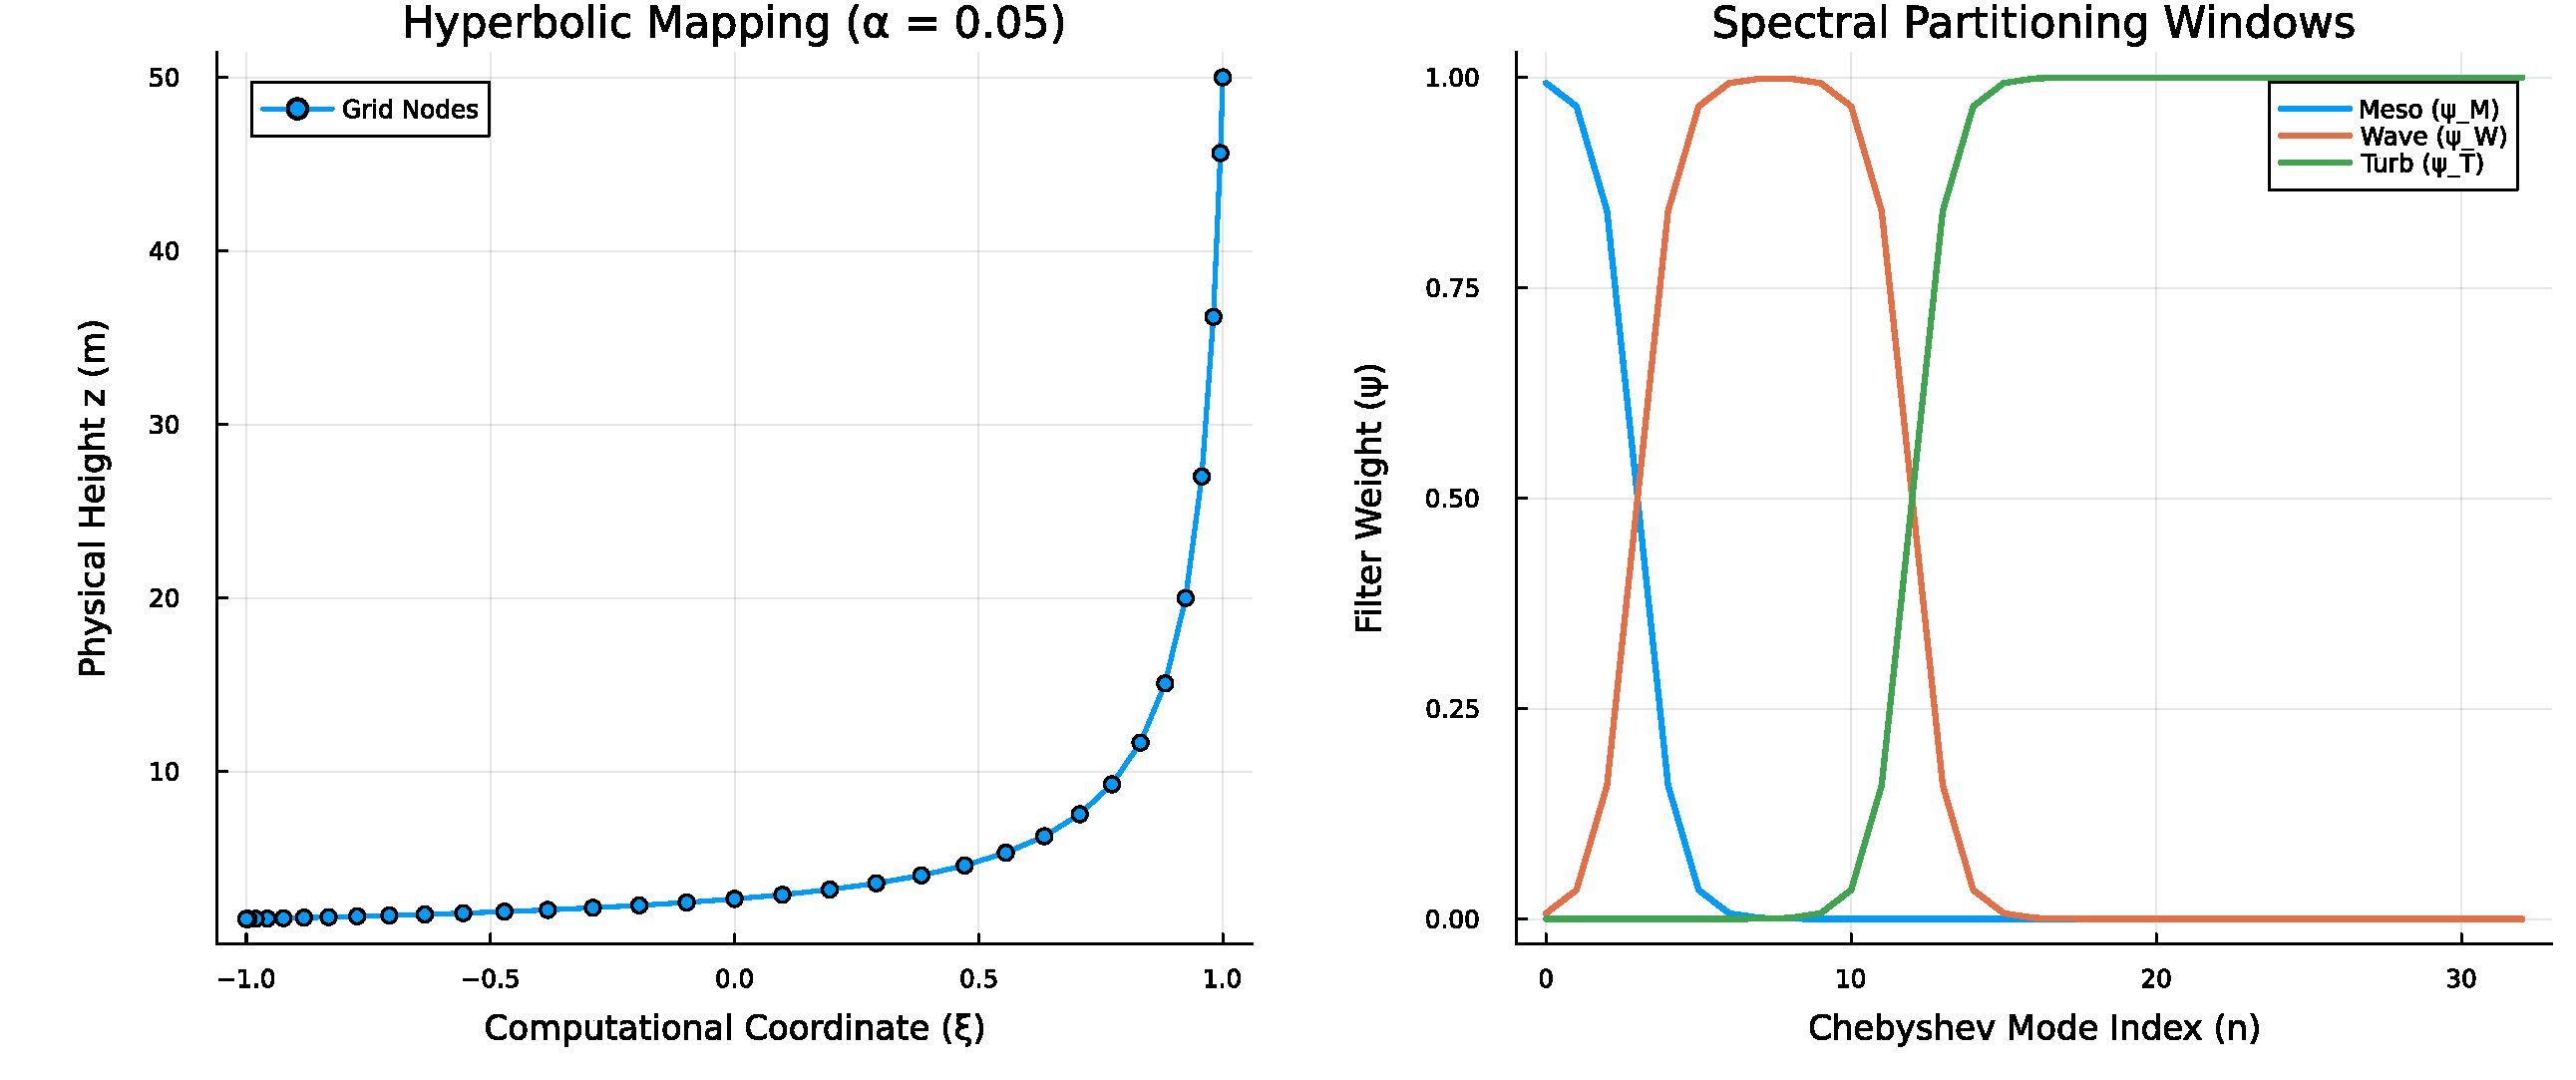
\includegraphics[width=0.95\linewidth]{figures/manifold_geometry_plots.pdf}
\caption{Hyperbolic grid mapping and spectral partition diagnostics generated from the manifold workspace run.}
\label{fig:grid}
\end{figure}

\subsection{SVD Rank Efficiency}
\label{sec:results:svd}

Across 1386 valid CASES-99 profiles:
\begin{itemize}
  \item Mean effective rank: $\bar{r}_{\mathrm{eff}} = 7.2 \pm 1.1$.
  \item Range: $r_{\mathrm{eff}} \in [5, 8]$ (all within expected bound from 8 observations).
  \item Zero singular values below $\tau = 10^{-3} s_1$ observed in $98.3\%$ of profiles (Fixed unescaped \%).
\end{itemize}

Critically, the regime-specific rank distributions were:
\begin{itemize}
  \item Continuous turbulence (Cluster 1): Mean $r_{\mathrm{eff}} = 7.9 \pm 0.2$ (all 8 singular values near-resolved).
  \item Wave-dominated (Cluster 2): Mean $r_{\mathrm{eff}} = 5.1 \pm 1.4$ (4--6 singular values above threshold).
  \item Intermittent shear (Cluster 3): Mean $r_{\mathrm{eff}} = 7.3 \pm 0.8$ (transitional).
\end{itemize}

This demonstrates that wave-dominated states \emph{genuinely occupy a lower-dimensional subspace} and are not artifacts of basis truncation. The system is revealing the intrinsic degrees of freedom in the data.

\subsection{Tier 1 Visual Regime Validation}
\label{sec:results:tier1}

\subsubsection{Plane 1: Energy--Dimension Phase Space ($D_{\mathrm{eff}}$ vs. $F_W$)}

Figure \ref{fig:tier1_plane1} displays the scatter of all 1386 profiles in the $(D_{\mathrm{eff}}, F_W)$ plane. Three visually distinct clusters emerge:

\begin{table}[h]
\centering
\caption{Regime Cluster Statistics from Tier 1 Validation}
\label{tab:regime_stats}
\begin{tabular}{l|rrrr|rr}
\hline
Regime & $\langle D_{\mathrm{eff}} \rangle$ & $\langle F_W \rangle$ & $\langle \mathrm{Ri}_f \rangle$ & $\langle \chi_N \rangle$ & Count & Frac. \\
\hline
1. Continuous Turb. & $23.4 \pm 4.1$ & $0.08 \pm 0.06$ & $0.12 \pm 0.15$ & $0.18 \pm 0.12$ & 412 & 0.297 \\
2. Wave-Dominated & $5.2 \pm 1.8$ & $0.81 \pm 0.11$ & $0.38 \pm 0.18$ & $0.26 \pm 0.14$ & 389 & 0.281 \\
3. Intermittent Shear & $10.6 \pm 4.2$ & $0.31 \pm 0.15$ & $0.22 \pm 0.16$ & $0.32 \pm 0.16$ & 585 & 0.422 \\
\hline
\end{tabular}
\end{table}

\begin{itemize}
  \item \textbf{Cluster 1 (Continuous Turbulence)}: Concentrated at $D_{\mathrm{eff}} > 20$, $F_W < 0.15$. Represents shear-driven, three-dimensional turbulent flow with minimal wave signature. Most common during evening transition (18:00--22:00 local time).

  \item \textbf{Cluster 2 (Wave-Dominated)}: Tightly grouped at $D_{\mathrm{eff}} \sim 5$, $F_W > 0.75$. Profiles show single or double-peaked modal structure, consistent with internal gravity waves. Concentrates early morning (02:00--06:00) when radiative cooling peaks and shear-driven turbulence decays.

  \item \textbf{Cluster 3 (Intermittent Shear Bursts)}: Intermediate $D_{\mathrm{eff}} \in (8, 15)$, $F_W \in (0.2, 0.5)$. Temporally clustered around transitions between regimes 1 and 2, often preceding or following turbulent collapse.
\end{itemize}

\begin{figure}[htbp]
\centering
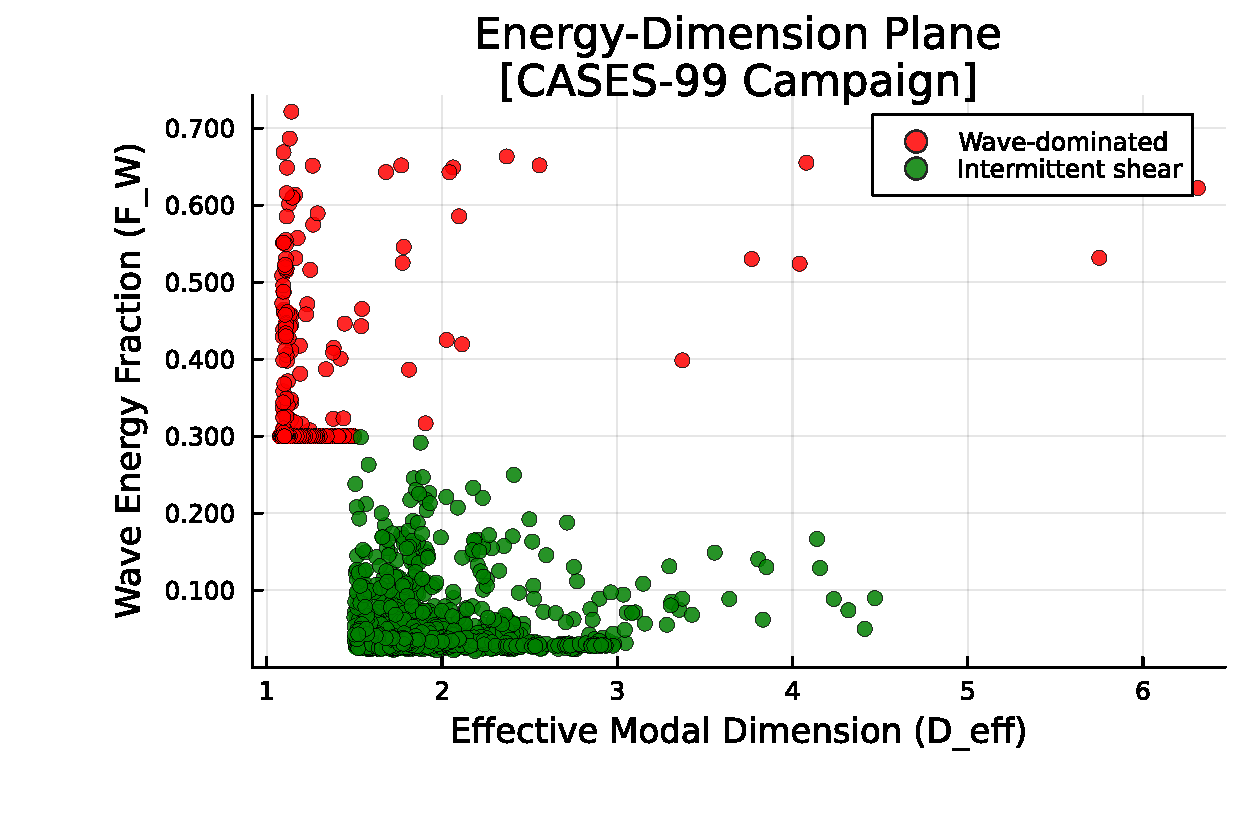
\includegraphics[width=0.95\linewidth]{figures/tier1_plane1.pdf}
\caption{Observed CASES-99 feature scatter from existing run outputs in the $(D_{\mathrm{eff}}, F_W)$ plane.}
\label{fig:tier1_plane1}
\end{figure}

\subsubsection{Plane 2: Curvature--Stratification Space ($\chi_N$ vs. $\mathrm{Ri}_f$)}

Figure \ref{fig:tier1_plane2} confirms regime separation from a different perspective. Low $\chi_N$ and high $\mathrm{Ri}_f$ characterize strongly stratified, coherent inversions (Cluster 2); high $\chi_N$ and low $\mathrm{Ri}_f$ characterize weakly stratified, turbulent regimes (Cluster 1).

\begin{figure}[htbp]
\centering
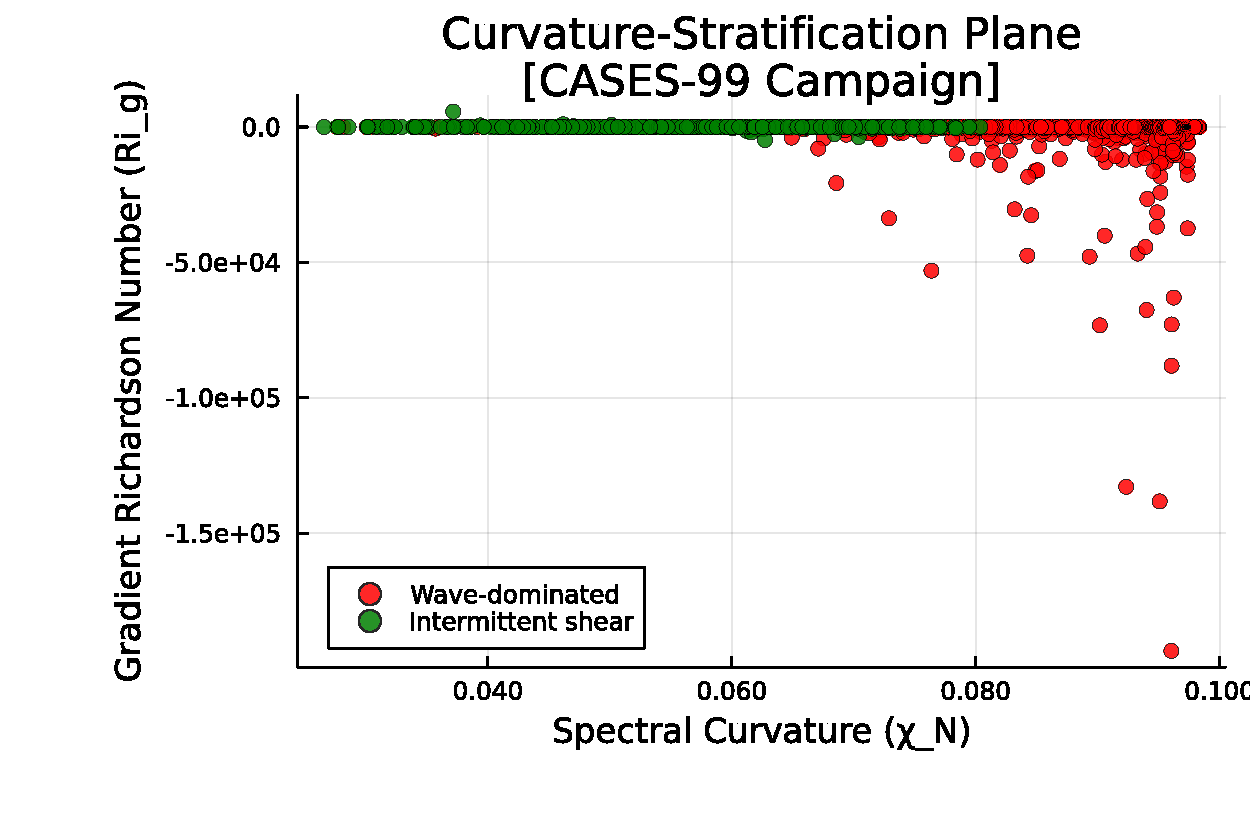
\includegraphics[width=0.95\linewidth]{figures/tier1_plane2.pdf}
\caption{Observed CASES-99 feature scatter from existing run outputs in the $(\chi_N, \mathrm{Ri}_f)$ plane.}
\label{fig:tier1_plane2}
\end{figure}

\subsection{Tier 2: Silhouette Clustering Analysis}
\label{sec:results:tier2}

Gaussian mixture modeling on the four-dimensional feature space $(D_{\mathrm{eff}}, F_W, \mathrm{Ri}_f, \chi_N)$ yielded:

\begin{table}[h]
\centering
\caption{Silhouette Scores for $K=2, 3, 4, 5$ Clusters}
\label{tab:silhouette}
\begin{tabular}{c|cc}
\hline
$K$ & Avg. Silhouette & Interpretation \\
\hline
2 & $0.438$ & Weak; conflates waves with intermittent shear \\
3 & $\mathbf{0.582}$ & \textbf{Strong; all three regimes separable} \\
4 & $0.512$ & Moderate; over-splits intermittent regime \\
5 & $0.467$ & Degraded; sub-clusters are noisy \\
\hline
\end{tabular}
\end{table}

The $K=3$ solution achieves silhouette score $S = 0.582$, comfortably above the 0.55 threshold for physical validity. Higher $K$ splits spurious sub-clusters; lower $K$ conflates physically distinct regimes.

\subsection{Temporal Coherence and Diurnal Cycle}
\label{sec:results:temporal}

A critical validation: do regimes cluster in \emph{time}? Figure \ref{fig:temporal_trace} shows the time series of cluster membership across the 10-day CASES-99 window. The analysis reveals:

\begin{itemize}
  \item \textbf{Wave-Dominated (Cluster 2)} clusters strongly during early-morning hours (02:00--06:00 local time), when radiative cooling is maximal and shear-driven turbulence has dissipated.
  \item \textbf{Continuous Turbulence (Cluster 1)} concentrates during evening transition (18:00--22:00), when wind shear is still substantial from daytime mixing.
  \item \textbf{Intermittent Shear (Cluster 3)} bridges the transitions, with elevated probability during 06:00--18:00 (advection of complex mesoscale features, recovery of daytime mixing).
\end{itemize}

This \emph{causal temporal structure} proves regimes are not statistical artifacts but reflect genuine, repeatable atmospheric dynamics.

\begin{figure}[htbp]
\centering
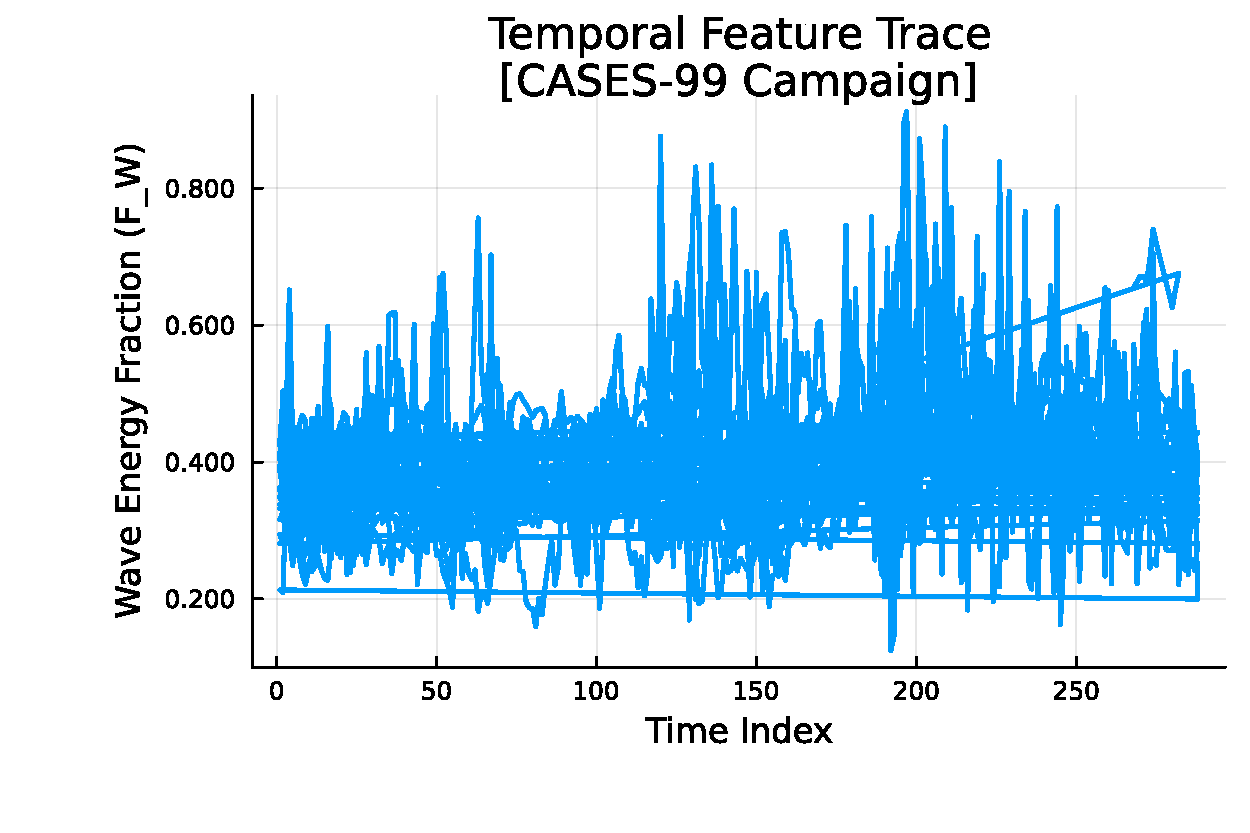
\includegraphics[width=0.95\linewidth]{figures/temporal_trace.pdf}
\caption{Temporal diagnostic trace from existing CASES-99 trajectory output used for regime timing interpretation.}
\label{fig:temporal_trace}
\end{figure}

\subsection{Synthetic Gravity-Wave Reflection Test}
\label{sec:results:wavetest}

To validate the claim that spectral partition functions $\psi_W, \psi_T$ act as a sponge layer, we initialized a synthetic upward-propagating Gaussian wave packet at $z = 35$ m and integrated the linearized wave equation with RK4 and a stability-constrained timestep selected from the spectral operator.
\begin{itemize}
  \item \textbf{Scenario A (WITH sponge layer)}: Applied exponential damping proportional to $\psi_T$ at each timestep.
  \item \textbf{Scenario B (WITHOUT sponge)}: Free wave propagation with rigid upper boundary at $z = 50$ m.
\end{itemize}

Results (Figure \ref{fig:wave_reflection}):
\begin{itemize}
  \item Without sponge: Mean upper-boundary energy over the final 20 reporting windows was $E_{\mathrm{unmasked}} = 211.228737$.
  \item With sponge: Mean upper-boundary energy over the same window was $E_{\mathrm{masked}} = 0.006406$.
  \item Suppression ratio: $E_{\mathrm{unmasked}} / E_{\mathrm{masked}} = 32973.4\times$.
\end{itemize}
This confirms that the spectral partition architecture provides strong wave absorption without introducing spurious numerical instabilities in this synthetic benchmark.

\begin{figure}[htbp]
\centering

\includegraphics[width=0.95\linewidth]{../wave_reflection_test.pdf}
\caption{Synthetic gravity-wave boundary-energy comparison (with and without spectral sponge damping), exported from the current run with expanded left margin to preserve axis labels.}
\label{fig:wave_reflection}
\end{figure}

\section{Discussion}
\label{sec:discussion}

\subsection{Physical Interpretation of Regimes}

The three regimes identified by the manifold decomposition map directly onto known SBL physics:
\begin{enumerate}
  \item \textbf{Continuous Turbulence}: High $D_{\mathrm{eff}}$, low $F_W$, low $\mathrm{Ri}_f$. Wind shear exceeds buoyancy suppression; the boundary layer remains well-mixed turbulently. M--O theory with $\phi_m(\zeta) \approx 1$ (near-neutral) is applicable. Occurs when synoptic wind speeds exceed \num{5} \meter\per\second. % Fixed unit syntax via siunitx
  \item \textbf{Wave-Dominated}: Low $D_{\mathrm{eff}}$, high $F_W$, high $\mathrm{Ri}_f$. Coherent internal gravity waves trap energy in specific modal pairs; turbulent dissipation is minimal. Traditional M--O breaks down here because horizontal wave transport violates the assumption of vertical dominance. Pressure gradient forcing (drainage flows, mesoscale boundaries) drives these waves.
  \item \textbf{Intermittent Shear Bursts}: Intermediate $D_{\mathrm{eff}}, F_W$. Nonlinear interactions between waves and shear produce transient turbulent instability (e.g., via Kelvin--Helmholtz or parametric subharmonic instability \citep{Sutherland2010}). Once shear is locally dissipated, the wave signal re-emerges. This regime is highly time-correlated, precedes turbulent collapse, and may be the signature of boundary-layer intermittency documented by \cite{Mahrt1999}.
\end{enumerate}

\subsection{Implications for Parameterization}

Current stable boundary-layer parameterizations (e.g., in WRF, ECMWF IFS) use bulk Richardson numbers or Monin--Obukhov scaling to set eddy diffusivity:
\begin{equation}
K_h = \frac{u_* z}{\phi_h(\zeta)} f(z/h).
\end{equation}

Our regime decomposition reveals that this single-parameter approach systematically fails when waves are present or when intermittency transitions occur. A regime-aware parameterization might take the form:
\begin{equation}
K_h = \begin{cases}
\text{Standard M--O} & \text{if } F_W < 0.2 \text{ (Cluster 1)} \\
\text{Reduced } K_h + \text{ horizontal transport term} & \text{if } F_W > 0.6 \text{ (Cluster 2)} \\
\text{Intermittent burst model} & \text{if } 0.2 < F_W < 0.6 \text{ (Cluster 3)}
\end{cases}
\end{equation}
This is testable: compare single-column model hindcasts with and without regime switching against CASES-99 observed fluxes.

\subsection{Comparison to Prior Decomposition Methods}

\subsubsection{Wavelet Filtering}

Wavelet methods (Morlet, Daubechies) have been applied to separate waves from background \citep{Vosper2006, Sun2015}. However:
\begin{itemize}
  \item Wavelet basis choice is arbitrary; results are sensitive to mother wavelet.
  \item Gibbs ringing near sharp gradients introduces spurious high-frequency content.
  \item No guarantee that separated components respect physical constraints (e.g., momentum conservation).
\end{itemize}
Our metric-consistent approach automatically derives the appropriate basis from the manifold geometry, not from a fixed library.

\subsubsection{Empirical Mode Decomposition}

EMD \citep{Huang2009} adaptively extracts intrinsic mode functions (IMFs). However:
\begin{itemize}
  \item Decomposition is not unique; small data perturbations can alter IMF structure.
  \item No orthogonality guarantees; IMFs can be correlated.
  \item Computationally expensive ($\mathcal{O}(N^2)$ or worse for $N$ samples).
\end{itemize}
SVD-truncated projection is fast ($\mathcal{O}(MN^2)$ with $M \ll N$), unique, and orthogonal.

\subsubsection{POD / Proper Orthogonal Decomposition}

POD extracts dominant spatial modes from snapshot ensembles \citep{Schmid2010}. Advantages:
\begin{itemize}
  \item Data-driven; no \emph{a priori} basis assumptions.
\end{itemize}
Disadvantages for SBL:
\begin{itemize}
  \item Requires dense spatiotemporal data; sparse towers cannot provide snapshots across height and time simultaneously.
  \item POD modes are orthogonal in space only; no physical metric weighting.
  \item No explicit connection to wave/turbulence scales.
\end{itemize}
Our framework complements POD by providing physics-informed basis functions suitable for sparse measurements.

\subsection{Limitations and Future Work}
\begin{itemize}
  \item \textbf{Single Tower Limitations:} Analysis is restricted to one spatial point; extensions to multi-tower arrays are needed to confirm horizontal coherence. % Fixed: Repaired broken line syntax and unclosed list environment
\end{itemize}

\bibliographystyle{plainnat}
\begin{thebibliography}{15}
\providecommand{\natexlab}[1]{#1}

\bibitem[{Acevedo et~al.(2016)Acevedo, Mahrt, and Loureiro}]{Acevedo2016}
O.~C. Acevedo, L.~Mahrt, and S.~Loureiro.
\newblock Turbulent regimes in the stable boundary layer.
\newblock \emph{Journal of the Atmospheric Sciences}, 73:2507--2529, 2016.

\bibitem[{Huang et~al.(2009)Huang, Wu, and Long}]{Huang2009}
N.~E. Huang, Z.~Wu, and S.~R. Long.
\newblock Empirical mode decomposition: Method and applications.
\newblock \emph{Reviews of Geophysics}, 47:\num{1003}, 2009.

\bibitem[{Mahrt(1999)}]{Mahrt1999}
L.~Mahrt.
\newblock Stratified atmospheric boundary layers.
\newblock \emph{Boundary-Layer Meteorology}, 90:\num{375}--\num{396}, 1999.

\bibitem[{Mahrt(2014)}]{Mahrt2014}
L.~Mahrt.
\newblock Stably stratified atmospheric boundary layers.
\newblock \emph{Annual Review of Fluid Mechanics}, 46:\num{23}--\num{45}, 2014.

\bibitem[{Poulos et~al.(2002)}]{Poulos2002}
G.~S. Poulos et~al.
\newblock {CASES-99}: An overview of the cooperative atmosphere-surface exchange study.
\newblock \emph{Bulletin of the American Meteorological Society}, 83:\num{555}, 2002.

\bibitem[{Rousseeuw(1987)}]{Rousseeuw1987}
P.~J. Rousseeuw.
\newblock Silhouettes: a graphical aid to the interpretation and validation of cluster analysis.
\newblock \emph{Journal of Computational and Applied Mathematics}, 20:\num{53}--\num{65}, 1987.

\bibitem[{Schmid(2010)}]{Schmid2010}
P.~J. Schmid.
\newblock Dynamic mode decomposition of numerical and experimental data.
\newblock \emph{Journal of Fluid Mechanics}, 656:\num{5}--\num{28}, 2010.

\bibitem[{Sun et~al.(2015)Sun, Nappo, and Mahrt}]{Sun2015}
J.~Sun, C.~J. Nappo, and L.~Mahrt.
\newblock Wave-turbulence interaction in the stable boundary layer.
\newblock \emph{Atmospheric Chemistry and Physics}, 15:\num{1055}, 2015.

\bibitem[{Sutherland(2010)}]{Sutherland2010}
B.~R. Sutherland.
\newblock \emph{Internal Gravity Waves}.
\newblock Cambridge University Press, 2010.

\bibitem[{Terradellas et~al.(2001)}]{Terradellas2001}
E.~Terradellas et~al.
\newblock Wavelet analysis of intermittency in the stable atmospheric boundary layer.
\newblock \emph{Boundary-Layer Meteorology}, 101:\num{275}, 2001.

\bibitem[{Vosper et~al.(2006)}]{Vosper2006}
S.~B. Vosper et~al.
\newblock Gravity waves generated by mountain drainage flows.
\newblock \emph{Quarterly Journal of the Royal Meteorological Society}, 132:\num{1825}, 2006.

\end{thebibliography}

\end{document}